%%%%%%%%%%%%%%%%%%%%%%%%%%%%%%%%%%%%%%
%%%%%%%%%%%%%%%%%%%%%%%%%%%%%%%%%%%%%%
% Do not edit the TeX file your work
% will be overwritten.  Edit the RnW
% file instead.
%%%%%%%%%%%%%%%%%%%%%%%%%%%%%%%%%%%%%%
%%%%%%%%%%%%%%%%%%%%%%%%%%%%%%%%%%%%%%



We consider the problem of clustering time-course gene expression data. 
While thousands of genes might be simultaneously 
measured in a given genomics experiment, 
many genes may exhibit similar expression patterns.  
Clustering gene expressions
is one way to reduce the dimensionality of a complex data set 
and to facilitate scientific interpretations of intricate biological processes. 
Often, such dimensionality reduction is used for exploratory analysis and
is a first step before further downstream investigation.  
It is important, therefore, to acertain the stability of the 
discovered clusters. 
 
We study a publicly available data set of mice gene expression
\citep{shoemaker:2015:ultrasensitive}.
Mice were infected with different influenza viruses, and expression levels of a set of genes were assessed at 14 time points after infection.
Our analysis focuses on mice treated with the ``A/California/04/2009'' strain. 
We normalize the data as described in
\citet{shoemaker:2015:ultrasensitive} and then apply the differential
analysis tool EDGE \citep{Storey:2005:significance} to rank the genes from most to least significantly differentially expressed. 
We fit a BNP model and run our analysis below on the top $\ngenes = 1000$ genes.

\subsubsection*{The model}

Each gene consists of $\ntimepoints = 42$ measurements of expression: three measurements (called biological replicates) at 14 unique timepoints.
The timepoints are unevenly spaced, with more frequent observations at the beginning. 
Following \citet{Luan:2003:clustering} we apply cubic B-splines to smooth the time course expression data. 
Specifically, we model the first 11 timepoints using
cubic B-splines with 7 degrees of freedom.
For the last three timepoints, $t = 72, 120, 168$ hours,
we use indicator functions. 
That is, if $\tilde \regmatrix$ is the design 
matrix where each column is a
B-spline basis vector evaluated at the $\ntimepoints$ measurement times, 
we append to $\tilde \regmatrix$ three additional columns: 
in these columns, entries are 1
if $t = 72, 120,$ or 168, repectively, and 0 otherwise. 
Call the full design matrix $\regmatrix$. 
We use indicators for the last three timepoints for numerical stability; 
without the indicator columns,
the matrix $\tilde \regmatrix^T \tilde \regmatrix$ is nearly singular
because the later timepoints are more spread out. 
See \figref{example_genes} for an example gene and the B-spline basis. 

%

\begin{knitrout}
\definecolor{shadecolor}{rgb}{0.969, 0.969, 0.969}\color{fgcolor}\begin{figure}[!h]

{\centering 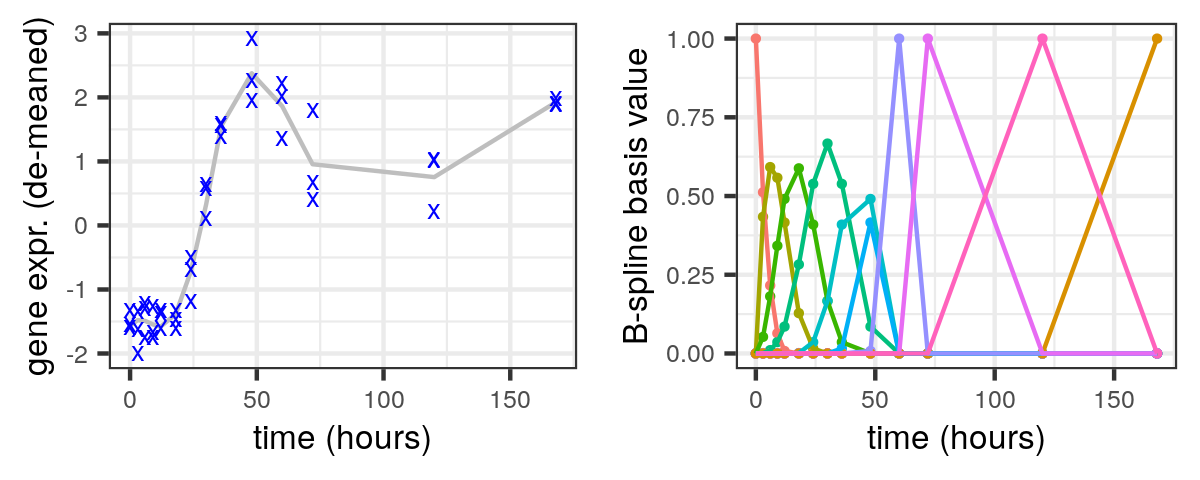
\includegraphics[width=0.980\linewidth,height=0.392\linewidth]{figure/example_genes-1} 

}

\caption[(Left) An example gene and its expression measured at 14 unique timepoints
    with three replicates at each timepoint.
     (Right) The cubic B-spline basis with 7 degrees of freedom, 
    along with three indicator functions for the last three timepoints, 
    $t = 72, 120, 168$]{(Left) An example gene and its expression measured at 14 unique timepoints
    with three replicates at each timepoint.
     (Right) The cubic B-spline basis with 7 degrees of freedom, 
    along with three indicator functions for the last three timepoints, 
    $t = 72, 120, 168$.}\label{fig:example_genes}
\end{figure}


\end{knitrout}
%


Let $\x_\n$ be the vector of observations for gene $\n$,
$(\x_{\n 1}, ..., \x_{\n \ntimepoints})^T$.
Each cluster is characterized by a vector of regression coefficients 
$\beta_k$ and a variance $\tau^{-1}_k$; 
the cluster parameters are $\theta_k = (\beta_k, \tau_k)$. 
The distribution of the data arising from cluster $k$ is 
\begin{align*}
p(\x_\n | \theta_k, \b_{n}) = 
\normdist{\x_\n | \regmatrix\beta_k + \b_{n},
\tau_k^{-1}I_{\ntimepoints \times \ntimepoints}},
\end{align*}
where $\b_{n}$ is a gene-specific additive offset. 
We include the additive offset because we 
are interested in clustering the pattern of gene expression, 
not the absolute level. 

The joint distribution can be written in the same form as~\eqref{bnp_model}, 
except that the conditional log-likelihood also conditions on $b_n$, 
and we also include an additional prior term:
\begin{align*}
\MoveEqLeft
\logp(\x, \theta, \z, \nu) ={}
\nonumber\\&
    \sum_{n=1}^N \sum_{k=1}^{\kmax}
        \z_{\n\k} \left(
            \logp(\x_n \vert \theta_\k, \b_n) + \logp(\b_n) + \log \pi_\k
        \right) +
    \sum_{k=1}^{\kmax} \left(
        \log \pstick(\nuk) + \logp(\theta_\k)
    \right).
\end{align*}
We use a normal prior for the shifts $\b_n$, 
a multivariate normal prior for the coefficients $\beta_n$,
and a gamma prior for the inverse variance $\tau$. 

Our variational distribution factorizes as~\eqref{vb_mf}
with the addition
of a factor for the additive shift: 
\begin{align*}
\q(\zeta \vert \eta) =
    \left( \prod_{\k=1}^{\kmax - 1} \q(\nuk \vert \eta) \right)
    \left( \prod_{\k=1}^{\kmax} \q(\theta_\k \vert \eta) \right)
    \left( \prod_{\n=1}^{\N} \q(\z_{\n} \vert \eta) 
    \q(\b_{\n} \vert \z_{\n}, \eta)\right).
\end{align*}
Note that the variational distribution for $\b_\n$ conditions on $\z$.
We set $\q(\b_{\n} \vert \z_{\n} = k, \eta)$ to be Gaussian
with variational parameters dependent on $\k$. 
For simplicity in this application,
we let $\q(\theta_\k \vert \eta) = \delta (\theta_k \vert \eta)$, 
where $\delta(\cdot \vert \eta)$ denotes a point mass at a parameterized location. 

By parameterizing 
$\q(\z_{\n}, \b_{\n} \vert \eta) = \q(\z_{\n} \vert \eta)  \q(\b_{\n} \vert \z_{\n}, \eta)$ 
the optimal variational parameters for $\q(\z_{\n}, \b_{\n} \vert \eta)$ 
have a closed form given $\q(\nu, \theta \vert \eta)$. See \secref{put_in_appendix}. Therefore, our model fits the global/local framework as discussed in ... 
\todo{need to work on a section that talks about this}

We fitted the initial approximate posterior at $\alpha_0 = 6$. 
\figref{gene_centroids} shows the inferred smoothers 
$\regmatrix\mathbb{E}_q[\beta_k]$ for selected clusters. 
\figref{gene_initial_coclustering} displays the inferred co-clustering matrix
$\coclusteringmatr(\eta)$, whose $(i,j)$-th entry is the
posterior probability that gene $i$ belongs to the same cluster
as gene $j$, given by 
\begin{align*}
\coclusteringmatr_{ij}(\eta) 
&= \expect{\q(\z\vert\eta)}{\ind{\z_{i} = \z_{j}}} \\
&= \sum_{k=1}^{\kmax}\left(\expect{\q(\z_i\vert\eta)}{\z_{ik}}
\expect{\q(\z_j\vert\eta)}{\z_{jk}}\right).
\end{align*}

Below, we evaluate the sensitivity of the inferred co-clustering matrix to 
both parametric and functional perturbations to the stick distribution. 


\begin{knitrout}
\definecolor{shadecolor}{rgb}{0.969, 0.969, 0.969}\color{fgcolor}\begin{figure}[!h]

{\centering 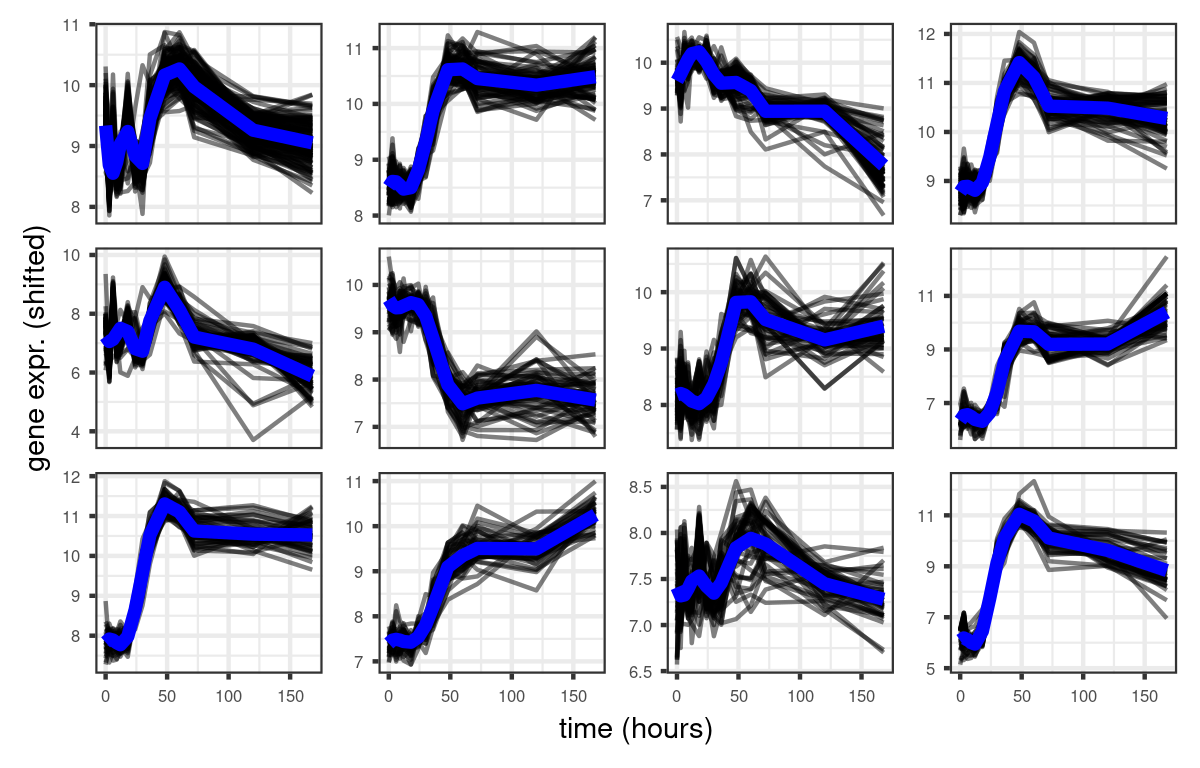
\includegraphics[width=0.980\linewidth,height=0.627\linewidth]{figure/gene_centroids-1} 

}

\caption[Inferred clusters in the mice gene expression dataset]{Inferred clusters in the mice gene expression dataset. 
    Shown are the top twelve most occupied clusters. 
    In blue, the inferred cluster centroid. 
    In grey, gene expressions averaged over replicates and
    shifted by their inferred intercepts. }\label{fig:gene_centroids}
\end{figure}


\end{knitrout}



\begin{knitrout}
\definecolor{shadecolor}{rgb}{0.969, 0.969, 0.969}\color{fgcolor}\begin{figure}[!h]

{\centering 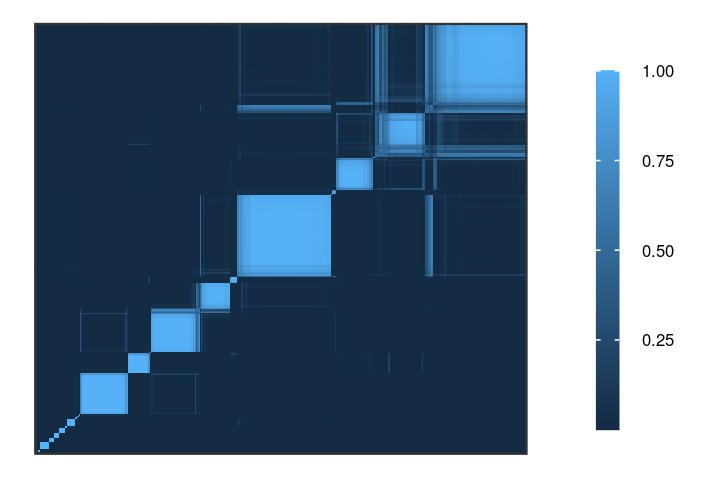
\includegraphics[width=0.588\linewidth,height=0.400\linewidth]{figure/gene_initial_coclustering-1} 

}

\caption[The inferred co-clustering matrix of gene expressions at $\alpha_0 = 6.$ ]{The inferred co-clustering matrix of gene expressions at $\alpha_0 = 6.$ }\label{fig:gene_initial_coclustering}
\end{figure}


\end{knitrout}


\subsubsection*{Sensitivity analysis}

We first evaluate the sensitivity of the co-clustering matrix $\coclusteringmatr$ 
to the choice of $\alpha$ in the
$\betadist{\nuk \vert 1, \alpha}$ stick distribution. 
Let $\coclusteringmatr_0 := \coclusteringmatr(\etaopt(\alpha_0))$ be the co-clustering matrix inferred at $\alpha_0$, 
and let $\Delta\coclusteringmatr(\eta) := 
\coclusteringmatr(\eta) - \coclusteringmatr_0$ be 
the difference in co-clustering matices after a change in the variational parameters $\eta$. 
We formed the linear approximation at $\alpha_0$ and computed
the change in co-clustering under the linearly approximated 
variational parameters, 
$\Delta\coclusteringmatr(\etalin(\alpha))$, at $\alpha = 1$ and $\alpha = 11$. 
For either $\alpha$, the change in the co-clustering matrix 
is miniscule (\figref{gene_alpha_coclustering}):
the largest entry of either matrix $\Delta\coclusteringmatr(\etalin(1))$ 
or $\Delta\coclusteringmatr(\etalin(11))$ is of order $10^{-2}$. 
Refitting the approximate posterior at $\alpha = 1$ and $\alpha = 11$ 
and computing $\Delta\coclusteringmatr(\etaopt(\alpha))$
confirms the insensitivity predicted by the linear approximation. 
Beyond capturing insensitivity, the linear approximation was also able to
approximate the sign and size of the changes in the individual entries of the coclustering matrix (these changes abeit small).  


\begin{knitrout}
\definecolor{shadecolor}{rgb}{0.969, 0.969, 0.969}\color{fgcolor}\begin{figure}[!h]

{\centering 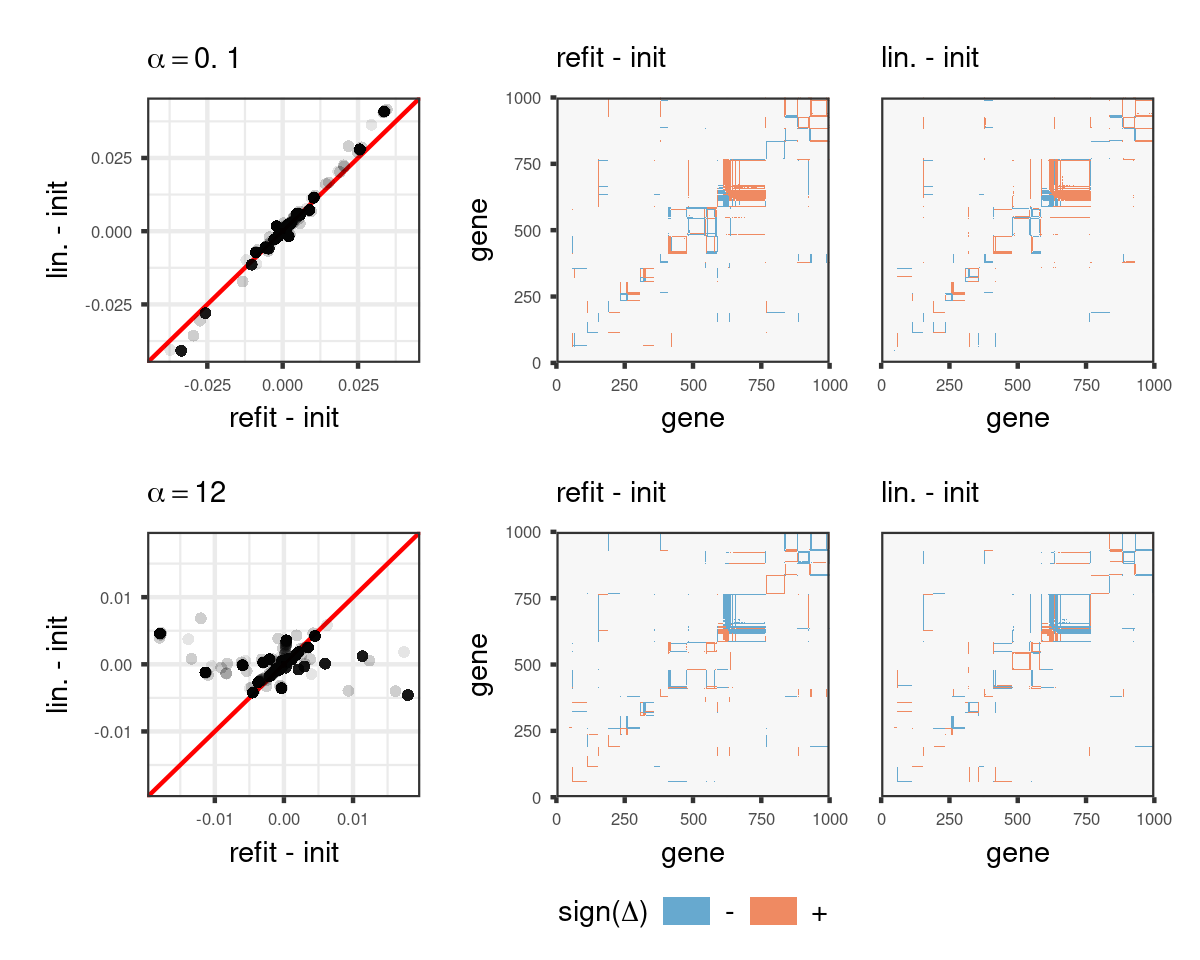
\includegraphics[width=0.980\linewidth,height=0.784\linewidth]{figure/gene_alpha_coclustering-1} 

}

\caption[Changes in the 
     co-clustering matrix at $\alpha = 1$ (top row)
     and $\alpha = 11$ (bottom row),
     relative to the co-clustering matrix at $\alpha_0 = 6$.
     The left column plots differences predicted by the
     linear approximation against differences from a model refit]{Changes in the 
     co-clustering matrix at $\alpha = 1$ (top row)
     and $\alpha = 11$ (bottom row),
     relative to the co-clustering matrix at $\alpha_0 = 6$.
     The left column plots differences predicted by the
     linear approximation against differences from a model refit; 
     each point represents an entry of the co-coclustering matrix.
     The middle and right columns display
     changes in the co-clustering matrix as obtained by the
     linear approximation and the model refit, respectively.
     For visualization, the differences in the heatmap 
     are clipped at $\pm 10^{-3}$. }\label{fig:gene_alpha_coclustering}
\end{figure}


\end{knitrout}


Insensitivity to $\alpha$ does not necessarily rule out insensitivity to other prior perturbations, however. 
As demonstrated in \secref{results_iris},
the influence function can provide guidance on which functional perturbations may result in greater sensitivity for a chosen posterior quantity. 
However, the co-clustering matrix as a posterior quantity is 
$\ngenes^2$-dimensional and 
thus does not lend itself to an easily interpretable influence function. 
We therefore summarize the co-clustering matrix into a scalar quantity: 
we use the sum of the eigenvalues of the symmetrically normalized graph Laplacian. 
This quantity has close connection with 
the number of distinct components in a graph CITE. 
Let this posterior quantity be denoted $\laplacianevsum$, given by 
\begin{align*}
  \laplacianevsum(\eta) = 
  \text{Tr}\left(
  I - D(\eta)^{-1/2} \coclusteringmatr(\eta) D(\eta)^{-1/2}
  \right),
\end{align*}
where $D(\eta)^{-1/2}$ is the diagonal matrix with entries $d_i = \sum_{j=1}^{\ngenes}[\coclusteringmatr(\eta)]_{ij}$. 
(And recall that the trace of a matrix is equivalent to the sum of its eigenvalues).

Because $\laplacianevsum(\eta)$ is a scalar quantity, we can plot its influence function. 
We choose a functional perturbation $\log\phi_{\textrm{ev}}$ that has a large, positive inner-product with the influence function.
In this case, we construct $\log\phi_{\textrm{ev}}$
using two Gaussian bumps aligned with
the two largest modes of the prior-weighted influence function
(\figref{gene_fpert_coclustering} top left). 
We anticipate $\log\phi_{\textrm{ev}}$
to have a large effect on $\laplacianevsum$. 
With $\laplacianevsum$ a proxy for our actual posterior quantity of interest, 
the full co-clustering matrix, we then expect that the co-clustering matrix 
will also experience large changes. 





Our intuition is confirmed in \figref{gene_fpert_coclustering}. 
After perturbing by $\log\phi_{\textrm{ev}}$, 
the largest changes in the co-clustering matrix are of now of order $10^{-1}$, 
an order of magnitude larger than the largest changes
after the $\alpha$ perturbations. 
The linear approximation again able to capture the qualitative changes in the co-clustering matrix after refitting at the perturbed prior. 


\begin{knitrout}
\definecolor{shadecolor}{rgb}{0.969, 0.969, 0.969}\color{fgcolor}\begin{figure}[!h]

{\centering 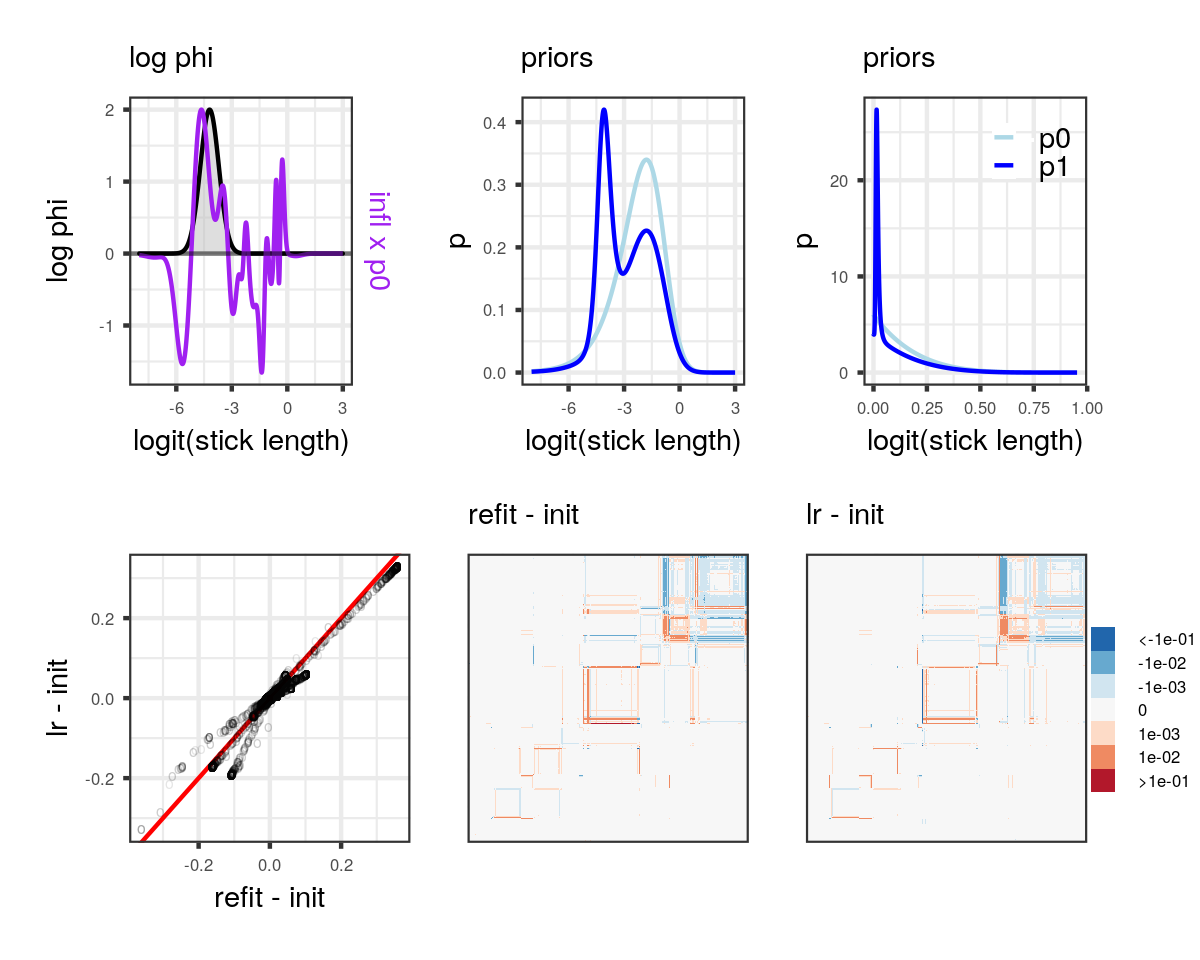
\includegraphics[width=0.980\linewidth,height=0.784\linewidth]{figure/gene_fpert_coclustering-1} 

}

\caption[Effect on the co-clustering matrix after a functional perturbation.
     The perturbation $\log\phi$ (top left, in grey) 
     is a difference of two Gaussian bumps 
     scaled to have L-infinity norm equal to two.
     $\log\phi$ is chosen such that the Gaussian bumps roughly align with the 
     two largest modes of the influence function]{Effect on the co-clustering matrix after a functional perturbation.
     The perturbation $\log\phi$ (top left, in grey) 
     is a difference of two Gaussian bumps 
     scaled to have L-infinity norm equal to two.
     $\log\phi$ is chosen such that the Gaussian bumps roughly align with the 
     two largest modes of the influence function. 
     The effect of this perturbation on the prior density in the top right. 
     The bottom row shows the effect of this perturbation on 
    the coclustering matrix.
    For visualization, the differences in the heatmap 
     are clipped at $\pm 10^{-1}$.}\label{fig:gene_fpert_coclustering}
\end{figure}


\end{knitrout}

The influence function is able to explain why the co-clustering matrix is 
insensitive to $\alpha$.
\figref{alpha_pert_logphi} shows the functional perturbation $\log\phi$ 
that corresponds to a change in $\alpha$, 
\begin{align*}
\log \phi_\alpha(\nu_k) :=
\log\betadist{\nu_k\vert 1, \alpha} -
\log\betadist{\nu_k\vert 1, \alpha_0},
\end{align*}
for $\alpha = 1$ and $\alpha = 11$.
These perturbations are large when the influence function is small. 
Hence, the inner product between the influence function and $\log\phi$ 
is small, and the linear approximation will predict small changes. 
The refitted results confirms the linear approximation predictions. 


\begin{knitrout}
\definecolor{shadecolor}{rgb}{0.969, 0.969, 0.969}\color{fgcolor}\begin{figure}[!h]

{\centering 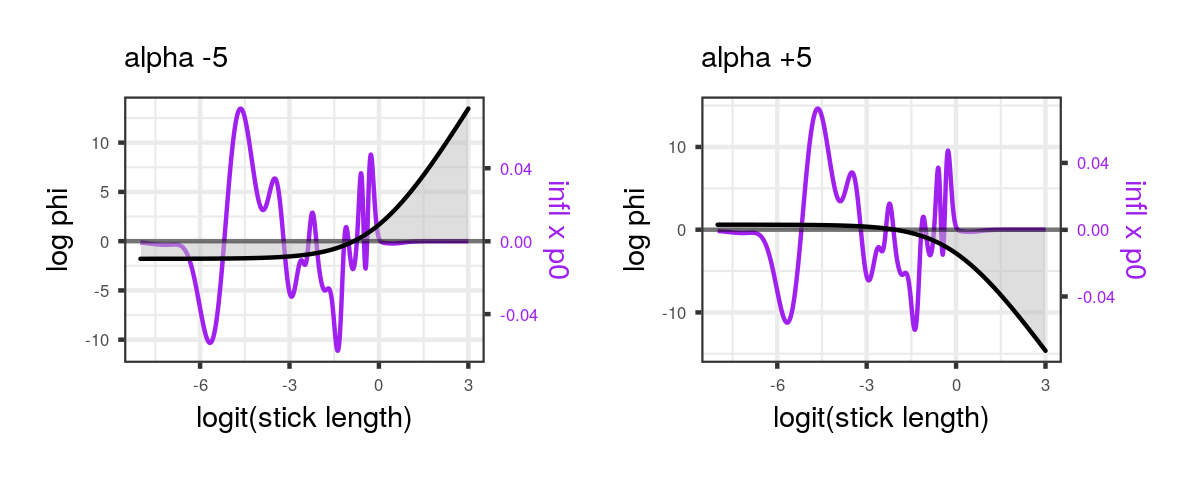
\includegraphics[width=0.980\linewidth,height=0.392\linewidth]{figure/alpha_pert_logphi-1} 

}

\caption[The log multiplicative perturbation $\log \phi_\alpha(\cdot)$ that 
    corresponds to decreasing the $\alpha$ parameter by five (left) or
    increasing the $\alpha$ parameter by five (right)]{The log multiplicative perturbation $\log \phi_\alpha(\cdot)$ that 
    corresponds to decreasing the $\alpha$ parameter by five (left) or
    increasing the $\alpha$ parameter by five (right). }\label{fig:alpha_pert_logphi}
\end{figure}


\end{knitrout}

Even with the selected functional perturbation however, 
the size of the differences in the co-clustering matrix remains modest. 
It is unlikely that any conclusions drawn from the co-clustering matrix would have changed after the prior perturbation. 
The co-clustering matrix appears insensitive to perturbations in the stick-breaking distribution. 

Finally, we note that the computational cost of the linear approximation is again favorable compared with refitting (\tabref{foo}). 
Forming the linear approximation, which requires a Hessian inversion, 
took 3-4 seconds; subsequent evaluations of $\etalin$ take milliseconds. 
Conversely, refitting the model can take up to 20 seconds. 

\begin{table}[tb]
\centering
\caption{Compute time of results on the mice data set. }
\tablabel{foo}
\begin{tabular}{|r|r|}
    \hline 
    & time (seconds) \\ 
    \hline 
    Initial fit & 30 \\
    \hline 
    Hessian solve for $\alpha$ sensitivity & 
        3.9\\
    Linear approx. $\eta^{lin}(\alpha)$ for $\alpha = 1$ & 
        0.0013\\
    Linear approx. $\eta^{lin}(\alpha)$ for $\alpha = 11$ & 
        0.0012\\
    Refit $\eta(\alpha)$ for $\alpha = 1$ & 
        14\\
    Refit $\eta(\alpha)$ for $\alpha = 11$ & 
        13\\
    \hline
    The influence function & 4.3\\ 
    Hessian solve for $\phi$ perturbation &
        3.3\\
    Linear approx. $\eta^{lin}(\epsilon)$ at $\epsilon = 1$ &
        0.00099\\
    Refit $\eta(\epsilon)$ at $\epsilon = 1$ &
        22\\
    \hline
\end{tabular}
\end{table}
